
% Font and layout
\usepackage{times}
\usepackage[margin=1in]{geometry}
\usepackage{titlesec}
\titleformat{\section}[block]{\huge\bfseries\centering\underline}{}{0em}{}
\setcounter{secnumdepth}{0}
\usepackage{color}
\usepackage{amsmath}
\usepackage{listings}
\renewcommand{\ttdefault}{lmtt}
\usepackage{xstring}

% Graphics and floats
\usepackage{graphicx}
\usepackage{float}
\usepackage{tikz}
\usepackage{grfext}
\usetikzlibrary{calc}
\usepackage{subcaption}


% Tables
\usepackage{booktabs}
\usepackage{array}
\usepackage{multirow}
\usepackage{longtable}
\usepackage{tabularx}
\usepackage{makecell}
\usepackage{ragged2e}
\usepackage[table]{xcolor}

% Custom column types
\newcolumntype{M}[1]{>{\centering\arraybackslash}m{#1}}
\newcolumntype{L}[1]{>{\raggedright\arraybackslash}m{#1}}

% Landscape support
\usepackage{pdflscape}
\usepackage{lscape}

% Code and Sweave
\usepackage{Sweave}

% CSV tables
\usepackage{csvsimple}

% TOC formatting
\usepackage{tocloft}
\usepackage{titletoc}
\renewcommand{\cftsecleader}{\cftdotfill{\cftdotsep}}

% Hyperlinks
\usepackage{hyperref}

% Page style and headers/footers
\usepackage{fancyhdr}
\usepackage{lastpage}
\pagestyle{fancy}
\fancyhf{}
\rhead{\thepage}
\lhead{Your Document Title or Section}
\renewcommand{\headrulewidth}{0.4pt}

% Horizontal rule command
\newcommand\HRule{\rule{\textwidth}{1pt}}

% Table Commands
\newcommand{\justiceTable}[2]{ % #1 = CSV file path, #2 = Caption
\begin{table}[H]
    \centering
    \renewcommand{\arraystretch}{1.5} % Add space between data rows
    \caption{#2}
    \vspace{2mm}
    \csvreader[
        tabular= {>{\centering\arraybackslash}p{0.25\textwidth} *{9}{>{\centering\arraybackslash}c}},
        table head = {
            \toprule
            \multicolumn{1}{c}{} &
            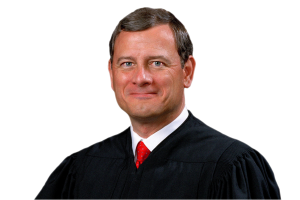
\includegraphics[width=1.75cm]{"images/justice_images/Roberts.png"} &
            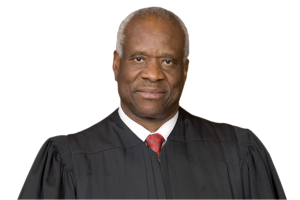
\includegraphics[width=1.75cm]{"images/justice_images/Thomas.png"} &
            
\includegraphics[width=1.75cm]{"images/justice_images/Alito.png"} &
            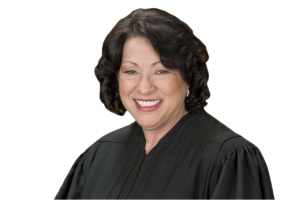
\includegraphics[width=1.75cm]{"images/justice_images/Sotomayor.png"} &
            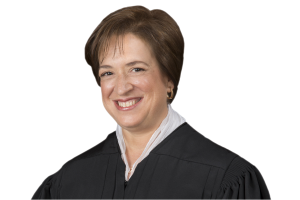
\includegraphics[width=1.75cm]{"images/justice_images/Kagan.png"} &
            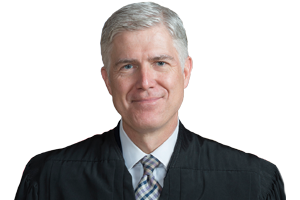
\includegraphics[width=1.75cm]{"images/justice_images/Gorsuch.png"} &
            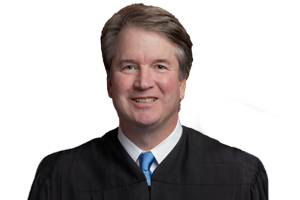
\includegraphics[width=1.75cm]{"images/justice_images/Kavanaugh.png"} &
            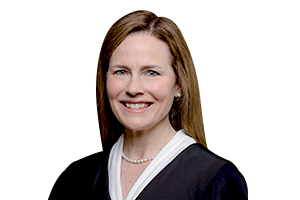
\includegraphics[width=1.75cm]{"images/justice_images/Barrett.png"} &
            
\includegraphics[width=1.75cm]{"images/justice_images/Jackson.png"} \rule[-2ex]{0pt}{0pt} \\[-2ex]
            \textbf{Case} & \textbf{Roberts} & \textbf{Thomas} & \textbf{Alito} & \textbf{Sotomayor} & \textbf{Kagan} & \textbf{Gorsuch} & \textbf{Kavanaugh} & \textbf{Barrett} & \textbf{Jackson} \\
            \cmidrule{1-10}
        },
        table foot = \bottomrule \\
    ]{#1}{}{
        \StrGobbleLeft{\csvcoli}{1}[\StrTemp]%
        \StrGobbleRight{\StrTemp}{1}[\CleanColi]%
        \normalsize \CleanColi & \csvcoliii & \csvcoliv & \csvcolv & \csvcolvi & \csvcolvii & \csvcolviii & \csvcolix & \csvcolx & \csvcolxi
    }
\end{table}
}  % Justice Participation


\newcommand{\attorneyWordsTime}[2]{ % #1 = CSV file path, #2 = Caption
\begin{table}[H]
    \centering
    %\renewcommand{\arraystretch}{1.5} % Add space between data rows
    \caption{#2}
    \vspace{2mm}
    \csvreader[
        tabular= {
            >{\centering\arraybackslash}p{0.25\textwidth}  % Case
            >{\centering\arraybackslash}p{0.15\textwidth}  % Docket
            >{\centering\arraybackslash}p{0.25\textwidth}  % Attorney
            >{\centering\arraybackslash}p{0.15\textwidth}  % Time
            >{\centering\arraybackslash}p{0.15\textwidth}  % Words
        },
        table head = {
            \toprule
            \textbf{Case} & \textbf{Docket} & \textbf{Attorney} & \textbf{Time} & \textbf{Words} \\
            \cmidrule{1-5}
        },
        table foot = \bottomrule \\
    ]{#1}{}{
        \csvcoli & \csvcolii & \csvcoliii & \csvcoliv & \csvcolv
    }
\end{table}
} % Attorney Participation


\newcommand{\attorneyEngagement}[2]{ % #1 = CSV file path, #2 = Caption
\begin{table}[H]
    \centering
    \caption{#2}
    \vspace{2mm}
    \csvreader[
        tabular= {>{\centering\arraybackslash}p{0.1\textwidth} >{\centering\arraybackslash}p{0.275\textwidth} *{10}{>{\centering\arraybackslash}p{0.09\textwidth}}},
        table head = {
            \toprule
            \multicolumn{1}{c}{} &
            \multicolumn{1}{c}{} &
            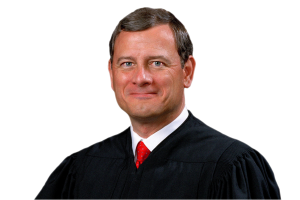
\includegraphics[width=1.75cm]{"images/justice_images/Roberts.png"} &
            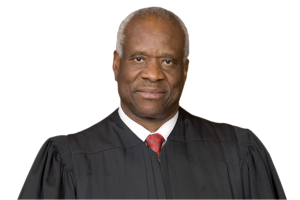
\includegraphics[width=1.75cm]{"images/justice_images/Thomas.png"} &
            
\includegraphics[width=1.75cm]{"images/justice_images/Alito.png"} &
            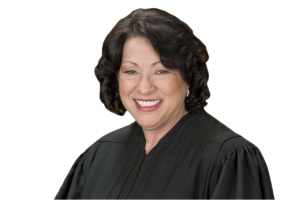
\includegraphics[width=1.75cm]{"images/justice_images/Sotomayor.png"} &
            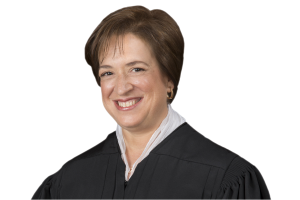
\includegraphics[width=1.75cm]{"images/justice_images/Kagan.png"} &
            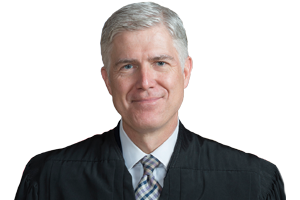
\includegraphics[width=1.75cm]{"images/justice_images/Gorsuch.png"} &
            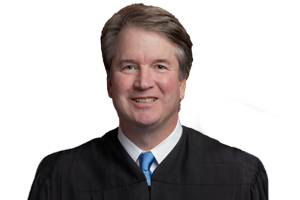
\includegraphics[width=1.75cm]{"images/justice_images/Kavanaugh.png"} &
            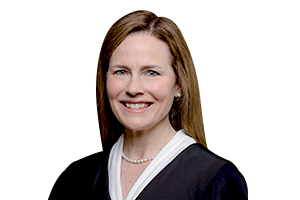
\includegraphics[width=1.75cm]{"images/justice_images/Barrett.png"} &
            
\includegraphics[width=1.75cm]{"images/justice_images/Jackson.png"} \rule[-2ex]{0pt}{0pt} \\[-2ex]
            \textbf{Docket} & \textbf{Attorney} & \textbf{Roberts} & \textbf{Thomas} & \textbf{Alito} & \textbf{Sotomayor} & \textbf{Kagan} & \textbf{Gorsuch} & \textbf{Kavanaugh} & \textbf{Barrett} & \textbf{Jackson} \\
            \cmidrule{1-11}
        },
        table foot = {
            \cmidrule{1-11}
            \multicolumn{11}{l}{\footnotesize \textit{Note}: Values represent total number of words by arguing attorney in response to particular Justice.} \\
            \bottomrule
        },
    ]{#1}{}{
        \normalsize \csvcolii & \csvcoliii & \csvcoliv & \csvcolv & \csvcolvi & \csvcolvii & \csvcolviii & \csvcolix & \csvcolx & \csvcolxi & \csvcolxii
    }
\end{table}
} % Attorney Engagement



\newcommand{\decisionInformation}[2]{ % #1 = CSV file path, #2 = Caption
\begin{table}[H]
    \centering
    \renewcommand{\arraystretch}{1.5} % Add space between data rows
    \caption{#2}
    \vspace{2mm}
    \csvreader[
        tabular= {>{\centering\arraybackslash}p{0.25\textwidth} *{7}{>{\centering\arraybackslash}p{0.107\textwidth}}},
        table head = {
            \toprule
            \textbf{Case} & \textbf{Docket} & \textbf{Date Argued} & \textbf{Date Decision} & \textbf{Lower Court} & \textbf{Decision} & \textbf{Author} & \textbf{Coalition} \\
            \cmidrule{1-8}
        },
        table foot = {
            \bottomrule
        },
    ]{#1}{}{
        \normalsize \csvcoli & \csvcolii & \csvcoliii & \csvcoliv & \csvcolv & \csvcolvi & \csvcolvii & \csvcolviii
    }
\end{table}
} % Decision Information


\newcommand{\voteMatrix}[2]{ % #1 = CSV file path, #2 = Caption
\begin{table}[H]
    \centering
    \renewcommand{\arraystretch}{1.5} % Add space between data rows
    \caption{#2}
    \vspace{2mm}
    \csvreader[
        tabular= {>{\centering\arraybackslash}p{0.35\textwidth} >{\centering\arraybackslash}p{0.1\textwidth} *{9}{>{\centering\arraybackslash}p{0.09\textwidth}}},
        table head = {
            \toprule
            \multicolumn{1}{c}{} &
            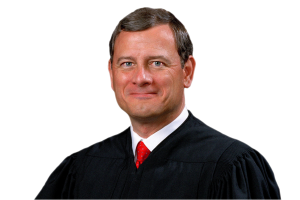
\includegraphics[width=1.75cm]{"images/justice_images/Roberts.png"} &
            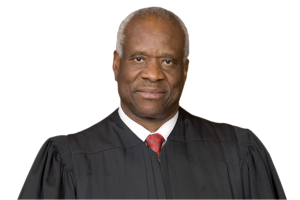
\includegraphics[width=1.75cm]{"images/justice_images/Thomas.png"} &
            
\includegraphics[width=1.75cm]{"images/justice_images/Alito.png"} &
            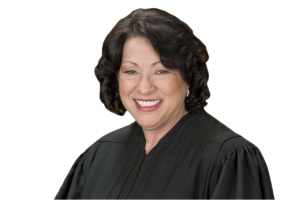
\includegraphics[width=1.75cm]{"images/justice_images/Sotomayor.png"} &
            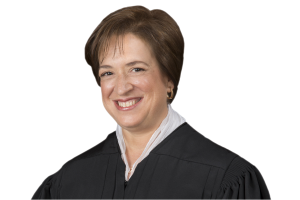
\includegraphics[width=1.75cm]{"images/justice_images/Kagan.png"} &
            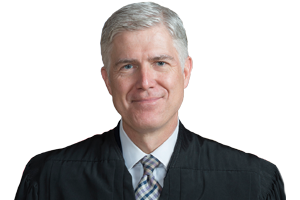
\includegraphics[width=1.75cm]{"images/justice_images/Gorsuch.png"} &
            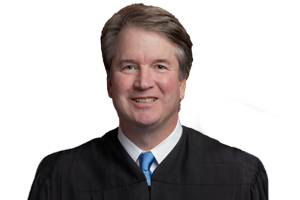
\includegraphics[width=1.75cm]{"images/justice_images/Kavanaugh.png"} &
            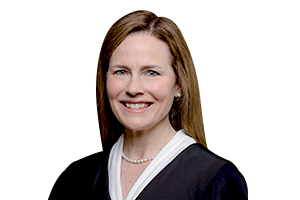
\includegraphics[width=1.75cm]{"images/justice_images/Barrett.png"} &
            
\includegraphics[width=1.75cm]{"images/justice_images/Jackson.png"} \rule[-2ex]{0pt}{0pt} \\[-2ex]
            \textbf{Case}  & \textbf{Roberts} & \textbf{Thomas} & \textbf{Alito} & \textbf{Sotomayor} & \textbf{Kagan} & \textbf{Gorsuch} & \textbf{Kavanaugh} & \textbf{Barrett} & \textbf{Jackson} \\
            \cmidrule{1-10}
        },
        table foot = {
            \midrule
            \multicolumn{10}{l}{\footnotesize M* = Majority Author; M = Majority Coalition; RC = Wrote Concurrence; JRC = Joined Regular Concurrence} \\
            \multicolumn{10}{l}{\footnotesize D = Wrote Dissent; JD = Joined Dissent; SC = Special Concurrence; DNP = Did Not Participate} \\
            \bottomrule
        },
    ]{#1}{}{
        \normalsize \csvcoli  & \csvcoliv & \csvcolv & \csvcolvi & \csvcolvii & \csvcolviii & \csvcolix & \csvcolx & \csvcolxi & \csvcolxii
    }
\end{table}
} % Vote Matrix



\newcommand{\circuitScorecard}[2]{ % #1 = CSV file path, #2 = Caption
\begin{table}[H]
    \centering
    \renewcommand{\arraystretch}{1.5} % Add space between data rows
    \caption{#2}
    \vspace{2mm}
    \csvreader[
        tabular= {>{\centering\arraybackslash}p{0.1\textwidth} *{6}{>{\centering\arraybackslash}p{0.14\textwidth}}},
        table head = {
            \toprule
            \textbf{Circuit} & \textbf{Affirm} & \textbf{Affirm \& Reverse} & \textbf{Reverse \& Remand} & \textbf{Reverse} & \textbf{Vacate \& Remand} & \textbf{DIG}  \\
            \cmidrule{1-7}
        },
        table foot = {
            \bottomrule
        },
    ]{#1}{}{
        \normalsize \csvcoli & \csvcolii & \csvcoliii & \csvcoliv & \csvcolv & \csvcolvii & \csvcolvi
    }
\end{table}
} % Circuit Scorecard


\newcommand{\termOpinionLengths}[2]{ % #1 = CSV file path, #2 = Caption
\begin{table}[H]
    \centering
    \renewcommand{\arraystretch}{1} % Add space between data rows
    \caption{#2}
    \vspace{2mm}
    \csvreader[
        tabular= {>{\centering\arraybackslash}p{0.5\textwidth} *{4}{>{\centering\arraybackslash}p{0.15\textwidth}}},
        table head = {
            \toprule
            \textbf{Case} & \textbf{Justice} & \textbf{Opinion} & \textbf{Word Count}   \\
            \cmidrule{1-4}
        },
        table foot = {
            \bottomrule
        },
    ]{#1}{}{
        \normalsize \csvcoli & \csvcolii & \csvcoliii & \csvcoliv
    }
\end{table}
} % Term Opinion Lengths


\newcommand{\termOpinionCounts}[2]{ % #1 = CSV file path, #2 = Caption
\begin{table}[H]
    \centering
    \renewcommand{\arraystretch}{1} % Add space between data rows
    \caption{#2}
    \vspace{2mm}
    \csvreader[
        tabular= {>{\centering\arraybackslash}p{0.25\textwidth} *{3}{>{\centering\arraybackslash}p{0.25\textwidth}}},
        table head = {
            \toprule
            \textbf{Justice} & \textbf{Majority} & \textbf{Concurrence} & \textbf{Dissent}   \\
            \cmidrule{1-4}
        },
        table foot = {
            \midrule
            \multicolumn{4}{l}{\footnotesize Note: \textit{Concurrence} includes Special Concurrences (In Part)} \\
            \bottomrule
        },
    ]{#1}{}{
        \normalsize \csvcoli & \csvcolii & \csvcoliii & \csvcoliv
    }
\end{table}
} % Term Opinion Counts


\newcommand{\comparisonOpinionCounts}[2]{ % #1 = CSV file path, #2 = Caption
\begin{table}[H]
    \centering
    \renewcommand{\arraystretch}{1} % Add space between data rows
    \caption{#2}
    \vspace{2mm}
    \csvreader[
        tabular= {>{\centering\arraybackslash}p{0.15\textwidth} *{4}{>{\centering\arraybackslash}p{0.15\textwidth}}},
        table head = {
            \toprule
            \textbf{Term} & \textbf{Justice} & \textbf{Majority} & \textbf{Concurrence} & \textbf{Dissent}   \\
            \cmidrule{1-5}
        },
        table foot = {
            \midrule
            \multicolumn{5}{l}{\footnotesize Note: \textit{Concurrence} includes Special Concurrences (In Part)} \\
            \bottomrule
        },
    ]{#1}{}{
        \normalsize \csvcoli & \csvcolii & \csvcoliii & \csvcoliv & \csvcolv
    }
\end{table}
} % Comparison Term Opinion Counts


\newcommand{\docketFilings}[2]{ % #1 = CSV file path, #2 = Caption
\begin{table}[H]
    \centering
    \renewcommand{\arraystretch}{1} % Add space between data rows
    \caption{#2}
    \vspace{2mm}
    \csvreader[
        tabular= {>{\centering\arraybackslash}p{0.25\textwidth} *{3}{>{\centering\arraybackslash}p{0.15\textwidth}}},
        table head = {
            \toprule
            \textbf{Period} & \textbf{Certiorari} & \textbf{Application} & \textbf{Motion}   \\
            \cmidrule{1-4}
        },
        table foot = {
            \bottomrule
        },
    ]{#1}{}{
        \normalsize \csvcoli & \csvcolii & \csvcoliii & \csvcoliv
    }
\end{table}
} % Cumulative & Monthly Variance in Docket Filings

\newcommand{\docketOrigins}[2]{ % #1 = CSV file path, #2 = Caption
\begin{table}[H]
    \centering
    \renewcommand{\arraystretch}{1} % Add space between data rows
    \caption{#2}
    \vspace{2mm}
    \csvreader[
        tabular= {>{\centering\arraybackslash}p{0.75\textwidth} *{1}{>{\centering\arraybackslash}p{0.25\textwidth}}},
        table head = {
            \toprule
            \textbf{Court} & \textbf{All Filings}    \\
            \cmidrule{1-2}
        },
        table foot = {
            \bottomrule
        },
    ]{#1}{}{
        \normalsize \RaggedRight \csvcoli & \csvcolii
    }
\end{table}
} % Docket Filings Origins


\newcommand{\circuitOrigins}[2]{ % #1 = CSV file path, #2 = Caption
\begin{table}[H]
    \centering
    \renewcommand{\arraystretch}{1} % Add space between data rows
    \caption{#2}
    \vspace{2mm}
    \csvreader[
        tabular= {>{\centering\arraybackslash}p{0.25\textwidth} *{3}{>{\centering\arraybackslash}p{0.15\textwidth}}},
        table head = {
            \toprule
            \textbf{Circuit} & \textbf{Certiorari} & \textbf{Application} & \textbf{Motion}   \\
            \cmidrule{1-4}
        },
        table foot = {
            \bottomrule
        },
    ]{#1}{}{
        \normalsize \csvcoli & \csvcolii & \csvcoliii & \csvcoliv
    }
\end{table}
} % Circuit Origins


\newcommand{\ifpPaid}[2]{ % #1 = CSV file path, #2 = Caption
\begin{table}[H]
    \centering
    \renewcommand{\arraystretch}{1} % Add space between data rows
    \caption{#2}
    \vspace{2mm}
    \csvreader[
        tabular= {>{\centering\arraybackslash}p{0.35\textwidth} *{1}{>{\centering\arraybackslash}p{0.35\textwidth}}},
        table head = {
            \toprule
            \textbf{Type} & \textbf{Count}  \\
            \cmidrule{1-2}
        },
        table foot = {
            \bottomrule
        },
    ]{#1}{}{
        \normalsize \csvcoli & \csvcolii
    }
\end{table}
} % IFP/PAID



\newcommand{\amiciVariance}[2]{ % #1 = CSV file path, #2 = Caption
\begin{table}[H]
    \centering
    \renewcommand{\arraystretch}{1} % Add space between data rows
    \caption{#2}
    \vspace{2mm}
    \csvreader[
        tabular= {>{\centering\arraybackslash}p{0.35\textwidth} *{1}{>{\centering\arraybackslash}p{0.35\textwidth}}},
        table head = {
            \toprule
            \textbf{No. Amici} & \textbf{Count}  \\
            \cmidrule{1-2}
        },
        table foot = {
            \bottomrule
        },
    ]{#1}{}{
        \normalsize \csvcoli & \csvcolii
    }
\end{table}
} % Amici Variance
